\documentclass[11pt]{article}

% ---------- Preamble ----------
\usepackage[margin=1in]{geometry}
\usepackage{hyperref}
\usepackage{graphicx}
\usepackage{booktabs}
\usepackage{xcolor}
\usepackage{enumitem}
\usepackage{titlesec}
\usepackage{listings}
\hypersetup{
  colorlinks=true,
  urlcolor=blue,
  linkcolor=black,
  citecolor=black
}

% Listings setup for R code
\lstdefinelanguage{R}{
  morekeywords={if, else, repeat, while, function, for, in, next, break},
  alsoletter={.},
  morekeywords=[2]{library,read_csv,View,mutate,rename,filter,select,arrange,
                   summarise,count,coalesce},
  sensitive=true,
  morecomment=[l]{\#},
  morestring=[b]",
}
\lstset{
  language=R,
  basicstyle=\ttfamily\small,
  keywordstyle=\color{blue!70!black},
  keywordstyle={[2]\color{purple!70!black}},
  commentstyle=\color{gray!70!black},
  stringstyle=\color{green!50!black},
  showstringspaces=false,
  columns=fullflexible,
  frame=single,
  breaklines=true,
  tabsize=2
}

\title{PS1: K-Drama Dataset Analysis}
\author{Barna Bose}
\date{September 7, 2025}

\begin{document}
\maketitle

\section*{Dataset}
\textbf{Source:} Kaggle / MyDramaList top-ranked Korean dramas.  
\textbf{File:} \texttt{kdrama.csv}

\bigskip

% -----------------------------------------------------------
\section*{Summary of Key Results}
\begin{center}
\begin{tabular}{@{}ll@{}}
\toprule
Total dramas (\#rows) & \textbf{250} \\
Variables (names) & 17 (see Q2) \\
Mean \# episodes & \textbf{19.064} \\
\# ratings $>$ 9 & \textbf{8} \\
Years 2020--2022 (inclusive) & \textbf{106} \\
Type of \texttt{Duration} & \texttt{character} \\
Netflix shows (exact match) & \textbf{12} \\
Avg.\ rating (Netflix exact) & \textbf{8.65} \\
\bottomrule
\end{tabular}
\end{center}

% -----------------------------------------------------------
\section*{Q1. How many Korean dramas are included?}
\begin{lstlisting}
library(readr)
kdrama <- read_csv("C:/Users/barna/Downloads/kdrama.csv")
nrow(kdrama)   # -> 250
\end{lstlisting}
\textbf{Answer:} 250

% -----------------------------------------------------------
\section*{Q2. List the variables in the dataset}
\begin{lstlisting}
names(kdrama)
\end{lstlisting}
\noindent
\textbf{Variables:}
\begin{enumerate}[itemsep=1pt, topsep=2pt]
\item Name
\item Aired Date
\item Year of release
\item Original Network
\item Aired On
\item Number of Episodes
\item Duration
\item Content Rating
\item Rating
\item Synopsis
\item Genre
\item Tags
\item Director
\item Screenwriter
\item Cast
\item Production companies
\item Rank
\end{enumerate}

% -----------------------------------------------------------
\section*{Q3. Mean total number of episodes}
\begin{lstlisting}
mean_episodes <- mean(na.omit(kdrama$`Number of Episodes`))
mean_episodes  # -> 19.064
\end{lstlisting}
\textbf{Answer:} 19.064

% -----------------------------------------------------------
\section*{Q4. Histogram of ratings}
\begin{lstlisting}
hist(kdrama$Rating,
     main = "Histogram of K-Drama Ratings",
     xlab = "Rating")
\end{lstlisting}

\begin{center}
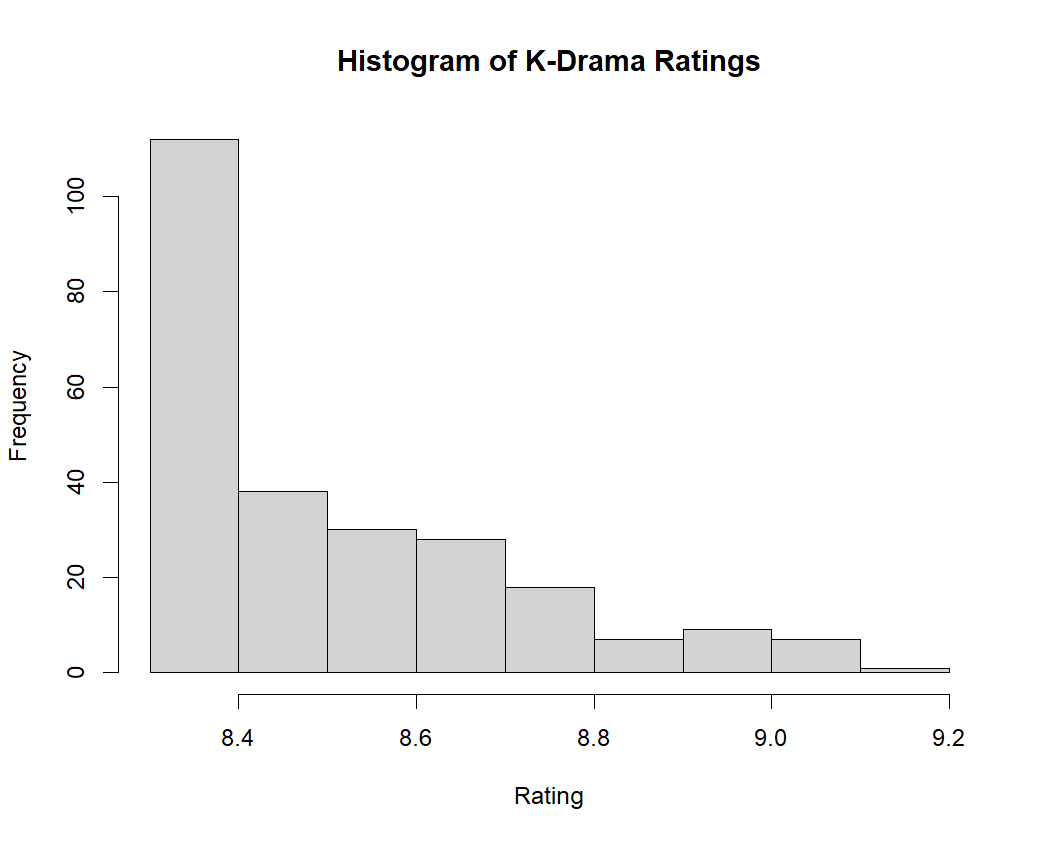
\includegraphics[width=.8\linewidth]{histogram of Kdrama.png} 
\end{center}

% -----------------------------------------------------------
\section*{Q5. How many shows have rating $>$ 9?}
\begin{lstlisting}
sum(kdrama$Rating > 9, na.rm = TRUE)  # -> 8
\end{lstlisting}
\textbf{Answer:} 8

% -----------------------------------------------------------
\section*{Q6. Rename \texttt{Year of release} to \texttt{Year} (in place)}
\begin{lstlisting}
library(dplyr)
kdrama <- kdrama %>% rename(Year = `Year of release`)

# Base-R alternative (3rd column):
# colnames(kdrama)[3] <- "Year"
\end{lstlisting}

% -----------------------------------------------------------
\section*{Q7. How many shows were released in 2020--2022?}
\begin{lstlisting}
sum(na.omit(kdrama$Year) >= 2020 & na.omit(kdrama$Year) <= 2022)  # -> 106
\end{lstlisting}
\textbf{Answer:} 106

% -----------------------------------------------------------
\section*{Q8. Type of \texttt{Duration}}
\begin{lstlisting}
class(kdrama$Duration)  # -> "character"
\end{lstlisting}
\textbf{Answer:} \texttt{character}

% -----------------------------------------------------------
\section*{Q9. Recode \texttt{Duration} to minutes; plot histogram}
Tidyverse (hours + minutes):
\begin{lstlisting}
library(dplyr)
library(stringr)

kdrama <- kdrama %>%
  mutate(Duration_min =
           coalesce(as.numeric(str_extract(Duration, "\\d+(?=\\s*hr)")), 0) * 60 +
           coalesce(as.numeric(str_extract(Duration, "\\d+(?=\\s*min)")), 0))

hist(na.omit(kdrama$Duration_min),
     main = "Histogram of Episode Duration (minutes)",
     xlab  = "Minutes")
\end{lstlisting}

\begin{center}
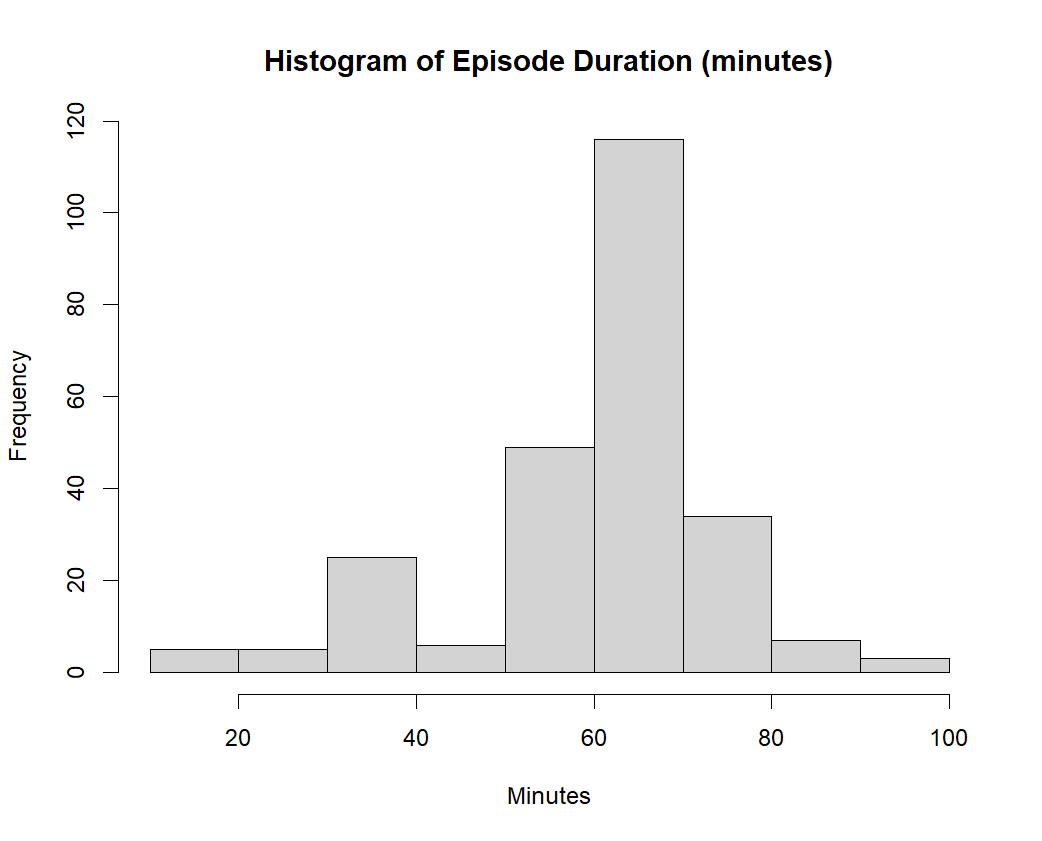
\includegraphics[width=.8\linewidth]{histogram of Duraton.png}
\end{center}


\begin{lstlisting}
(Extra Work) Base-R function approach 
Duration_to_minutes <- function(x) {
  hrs  <- ifelse(grepl("hr",  x, ignore.case=TRUE),
                 as.numeric(sub(".*?(\\d+)\\s*hr.*",  "\\1", x)), 0)
  mins <- ifelse(grepl("min", x, ignore.case=TRUE),
                 as.numeric(sub(".*?(\\d+)\\s*min.*", "\\1", x)), 0)
  hrs[is.na(hrs)]   <- 0
  mins[is.na(mins)] <- 0
  60*hrs + mins
}
\end{lstlisting}

% -----------------------------------------------------------
\section*{Q10. Subset to Netflix (exact match)}
\begin{lstlisting}
library(dplyr)
library(stringr)

netflix_exact <- kdrama %>%
  filter(str_trim(`Original Network`) == "Netflix")

nrow(netflix_exact)  # -> 12
\end{lstlisting}
\textbf{Answer:} 12 shows.

% -----------------------------------------------------------
\section*{Q11. Average rating for Netflix originals}
\begin{lstlisting}
mean(na.omit(netflix_exact$Rating))        # -> 8.65
# or:
mean(netflix_exact$Rating, na.rm = TRUE)   # -> 8.65
\end{lstlisting}
\textbf{Answer:} 8.65

\bigskip
\hrule
\bigskip

\end{document}

